\chapter{A search for new phenomena}
\label{chapter:2ljets}

\begin{epigraphs}
\qitem{%
An experiment is never a failure solely because it fails to
achieve predicted results. An experiment is a failure only when it also
fails adequately to test the hypothesis in question, when the data it
produces don’t prove anything one way or another.%
}%
{Robert M. Pirsig~\cite{pirsig1999zen}}
\qitem{%
But there is one feature I notice that is generally missing in cargo cult
science. \ldots\
% That is the idea that we all hope you have learned in studying science in
% school--we never say explicitly what this is, but just hope that you catch
% on by all the examples of scientific investigation. It is interesting,
% therefore, to bring it out now and speak of it explicitly.
It's a kind of scientific integrity, a principle of scientific thought that
corresponds to a kind of utter honesty --- a kind of leaning over backwards.%
}%
{Richard Feynman~\cite{feynman1974cargo}}
\end{epigraphs}


\begin{figure}[tp]
\centering
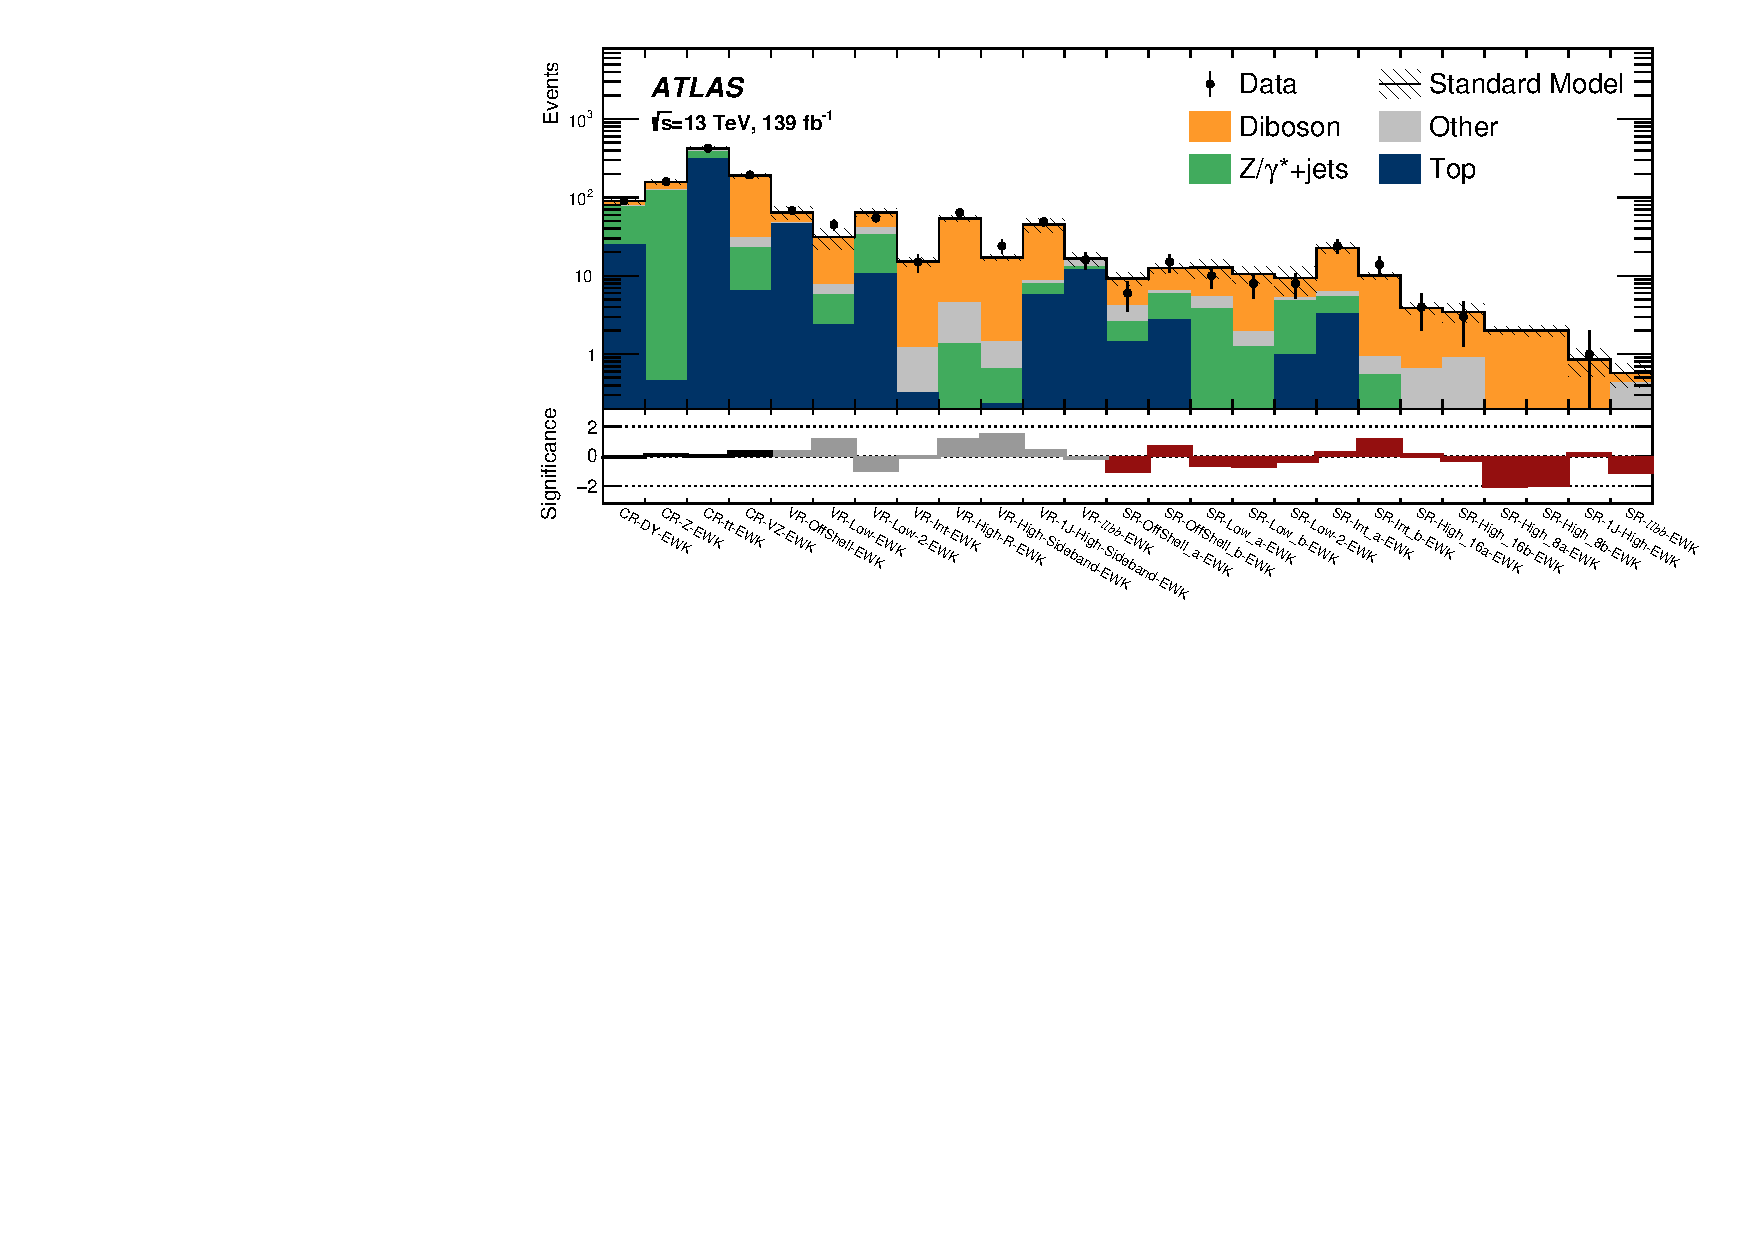
\includegraphics[width=\textwidth]{figures/2ljets_summary_log.pdf}
\caption{%
Data of the $\twoljets$ electroweak analysis with \emph{post-fit} backgrounds
for which the lower panel shows $S_\mathrm{ATLAS}$ from
Equation~\ref{eqn:significance_atlas}.
Control, validation and signal regions are shown from left to right, with the
regions within each category ordered approximately by their typical $\ptmiss$.
The `Top' category contains $t\bar t$ and $tW$ processes, and
`Other' contains fake/non-prompt lepton, higgs, triboson, , $t\bar tZ$ and other
rare top processes.%
}
\label{fig:ewk_summary}
\end{figure}



